\documentclass[aspectratio=1610]{beamer}

\usepackage{amsmath}
\usepackage{multirow}
\usepackage{url}
\usepackage{hyperref}

\hypersetup{
colorlinks=false,
}

\usepackage{listings,calc,graphicx}

\title % [short title] (optional, use only with long paper titles)
{CPSC 1000: Introduction to Computer Science}

\subtitle{by making Arduino projects} % (optional)

\author{Robert Benkoczi, C556\\\url{robert.benkoczi@uleth.ca}}
\date{11-Sep-2018}

% for figures created with IPE
%\pdfpagebox5

\lstloadlanguages{C}
\lstset{language=C,tabsize=2,aboveskip=-22pt,belowskip=-22pt,keepspaces,
  basicstyle=\small\ttfamily,}


\begin{document}

\begin{frame}[plain]
\titlepage
\end{frame}


%%%%%%

\begin{frame}[t,plain]{Course goals}

  At the end of the course, students will know to make Arduino projects.

  \smallskip
  See ``Arduino'' on youtube.

\end{frame}


%%%%%%

\begin{frame}[t,plain]{What is an Arduino?}

\hfill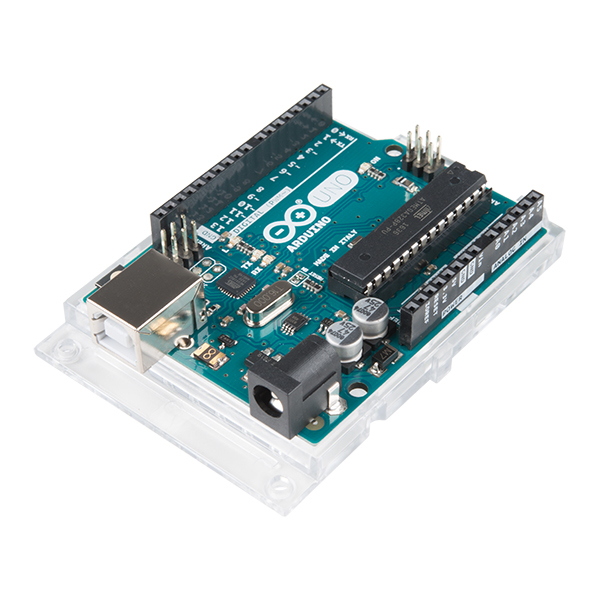
\includegraphics[width=0.3\textwidth]{figs/1-arduino.jpg}

\end{frame}

%%%%%%

\begin{frame}[t,plain]{Course content}

\begin{itemize}
\item Programming an Arduino micro-controller.
\item Process input from sensors.
\item Generating signals.
\end{itemize}

\end{frame}

%%%%%%


\begin{frame}[t,plain]{Week 1 lecture objectives}
To learn some basic programming for the Arduino micro-controller. 
\begin{itemize}
\item Functions / procedures.
\item Communication through the serial interface.
\item Expressions and arithmetic operations.
\item Variables.
\item Branching, if statements.
\item Repetition.
\end{itemize}

\smallskip
Arduino simulator:
\url{tinkercad.com}
\end{frame}


%%%%%%

\begin{frame}[t,plain]{Functions \& communication}

\end{frame}


%%%%%%

\begin{frame}[t,plain]{Expressions}

\end{frame}

%%%%%%

\begin{frame}[t,plain]{Variables}

\end{frame}


\end{document}
